%% BUICS THESIS STYLE for LaTeX2e
%%
%% badwanpk, Tue March 10 18:53:15 2015
%%
%% PLEASE send improvements to badwanpk at bui dot edu dot pk
%%
%%========================================
%% Commands: pdflatex tese
%%           bibtex tese
%%           makeindex tese (only if creating an index) 
%%           pdflatex tese
%%========================================

\documentclass[11pt,a4paper,oneside,openright]{report}
\usepackage[utf8]{inputenc}
\usepackage[english]{babel}
%\usepackage[portuges]{babel}
\usepackage{fancyvrb}
\usepackage{multirow}
%\usepackage{epstopdf}
\usepackage{rotating}
\usepackage{slashbox,pict2e}
\usepackage{soul}
\usepackage{amssymb}
\usepackage{lscape}
\usepackage{longtable}
\usepackage{makeidx}
\usepackage{amsmath}
\usepackage{multirow}
\usepackage{makecell}
\usepackage{wrapfig}


%% For the final version, comment next line and uncomment the second line
%\usepackage[provisional,alpharefs]{buics}
\usepackage[numericrefs]{buics} %alpharefs
\usepackage[utf8]{inputenc}

 %PDF properties 
\hypersetup{
pdftitle = {Title goes here...},
pdfauthor = {Author name},
		pdfsubject={Subject...},
    pdfcreator={MiKTex 2.9},
    pdfproducer={MiKTex 2.9},
    pdfkeywords = {Keywords},
    %pdfstartview={FitH},%fits the width of the page to the window
		pdfinfo={
    AuthorNameEnrollment1={AuthorName (Enrollment)},
		%AuthorNameEnrollment2={AuthorName (Enrollment)},%%uncomment this line if 2 authors
		Supervisor={SupervisorName (Designation)},
    Session={Fall 2015},%%Session in which the defense was arranged (Spring / Fall 20XX)
		InternalExaminer={Dr. ABC (Designation)},
		ExternalExaminer={Dr. XYZ (Designation)},
		ProjectCoordinator={Dr. XYZ (Designation)},
		HOD={Dr. XYZ (Designation)},
		DefenseDate={\today},
  }
}

%% Options: 
%% - english: titles, etc in english
%% - provisional: the thesis has not been approved yet
%% - print: links are not shown (for paper versions)
%% - alpharefs: bibliography references are alphabetic
%% - numericrefs: bibliography references are numbered (in order of citation)
%% ( by default: author-date format of the ``natbib'' package is used 


%% Provide a version number in order to keep track of
%% thesis versions (it will printed in the footer of most pages)

\version{v1.12.2015}




%% uncomment in the final version in order to make version footer disappear
%\noversiontrue

%% uncomment to create an index (at the end of the document)
\makeindex 





%%  path to the figures directory
%%  TIP: use folder ``figures'' to keep all your figures
\graphicspath{{figures/}}

%%----------------------------------------
%% TIP: if you want to define more macros, use an external file to
%% keep them
%some macro definitions

% format
\newcommand{\class}[1]{{\normalfont\slshape #1\/}}

% entities
\newcommand{\Feup}{Faculdade de Engenharia da Universidade do Porto}

\newcommand{\svg}{\class{SVG}}
\newcommand{\scada}{\class{SCADA}}
\newcommand{\scadadms}{\class{SCADA/DMS}}

%%----------------------------------------

%%========================================
%% Start of document
%%========================================
\begin{document}

%%----------------------------------------
%% Information about the work
%%----------------------------------------
\title{title}

\author{{\sc author name}\\Enrollment\\
{\sc author name}\\Enrollment    %%%uncomment this line if there is a second author
}


\degree{\textbf{\Large{Bachelor of Science in Computer Science}}}

%\degree{\emph{Thesis submitted to the Department of Computer Science, Bahria University, Islamabad\\for fulfillment of the requirements of Bachelors of Science in Computer Science degree.}}
%% Date of submission

\department{Department of Computer Science\\Bahria University, Islamabad}
\thesisdate{October 2025}
%\thesisdate{\Large{\textbf{September 2012}}}

%% insert copyright text if used
%\copyrightnotice{Author Name, 2025}

%% uncomment next line if necessary
\supervisor{Supervisor}{supervisor name}{}% {(Title)}
\supervisor{Co-Supervisor}{co supervisor name}{}%{(Title)}

% uncomment committee stuff in the final version if used

\certificatetext{We accept the work contained in the report titled ``TITLE OF THE REPORT'', written by Mr. AUTHOR1 NAME  AND Mr. AUTHOR2 NAME as a confirmation to the required standard for the partial fulfillment of the degree of Bachelor of Science in Computer Science.}

\committeetext{Approved by \ldots:}

\committeemember{Supervisor}{}{}
\signature
\committeemember{Internal Examiner}{}{}
\signature
\committeemember{External Examiner}{}{}
\signature
\committeemember{Project Coordinator}{}{}
\signature
\committeemember{Head of the Department}{}{}
\signature
%\committeedate{October, 2025}

%% specify cover logo (in folder ``figures'')
\logo{BUI-Logo}

%%----------------------------------------
%% Cover page(s)
%%----------------------------------------
\maketitle
%% uncomment next line in the final version if used
\committeepage

%% Preliminary materials
\StartPrelim
\begin{singlespace}
  \chapter*{Abstract}
\addcontentsline{toc}{chapter}{Abstract}
\lipsum % the abstract
  \chapter*{Acknowledgments}
%\addcontentsline{toc}{chapter}{Acknowledgments}

\lipsum

\vspace{10mm}


\flushleft{\textsc{Author Name}\\Bahria University \\E-8, Islamabad, Pakistan}

\flushleft{October 2025}  % the acknowledgments
  \cleardoublepage
  \pdfbookmark[0]{Table of Contents}{contents}
  \tableofcontents
  \cleardoublepage
  \pdfbookmark[0]{List of Figures}{figures}
  \listoffigures
  \cleardoublepage
  \pdfbookmark[0]{List of Tables}{tables}
  \listoftables
  \chapter*{Acronyms and Abbreviations}
%\addcontentsline{toc}{chapter}{Abbreviations}
\chaptermark{Acronyms and Abbreviations}

\begin{flushleft}
\begin{tabular}{l p{0.8\linewidth}}
%Remove the following and add yours.
DSA&	Data Structure and Algorithms\\
OOP	&Object Oriented Programming\\
PF	&Programming Fundamentals\\
SE	&Software Engineering\\
SQL	&Structured Query Language\\
UNESCO&	United Nations Educational, Scientific and Cultural Organization\\
UNICODE&	Unique, Universal, and Uniform Character enCoding\\
XML	&Extensible Markup Language\\

\end{tabular}
\end{flushleft}

  % the list of abbreviations used
\end{singlespace}

%%----------------------------------------
%% Body
%%----------------------------------------
\StartBody

%% TIP: use a separate  file for each
\chapter{Introduction} \label{chap:intro}

%\version{v1.11.2015}

\section*{}
\section{Is computer science science?}
Is computer science, science? Yes, it is \cite{ICSS05}.

This is one of the most important chapters of the report. It should begin with a clear statement of what the project is about so that the nature and scope of the project can be understood by any reader. It should summarise everything you set out to achieve, provide a clear summary of the project's background, relevance and main contributions. The introduction should set the context for the project and should provide the reader with a summary of the key things to look out for in the remainder of the report. When detailing the contributions it is helpful to provide pointers to the section(s) of the report that provide the relevant technical details. The introduction itself should be largely non-technical. It is useful to state the main objectives of the project as part of the introduction. Should have the following headings:

\begin{itemize}
	\item Project Background/Overview
	\item Problem Description
	\item 	Project Objectives 
	\item Project Scope
\end{itemize}

\section{The Degree Project Report}
The project report is an extremely important aspect of the degree project. It should be properly structured and contain all the necessary and appropriate information regarding the project.
 
Project report has to be progressively developed as and when various stages of project are completed and last few weeks should be used to bring it together as a coherent document.

\textbf{A well structured and consistently formatted project report makes reading easier and is suggestive of a careful and professional attitude towards its preparation. }

Remember that quantity does not automatically guarantee quality. A 150 page report is not twice as good as a 75-page one, nor a 10,000 line implementation twice as good as a 5,000 line one. Conciseness, clarity and elegance are invaluable qualities in report writing, just as they are in programming, and will be rewarded appropriately. 

This document provides various guidelines for preparing a well structured project report.

\begin{figure}[t]
\centering
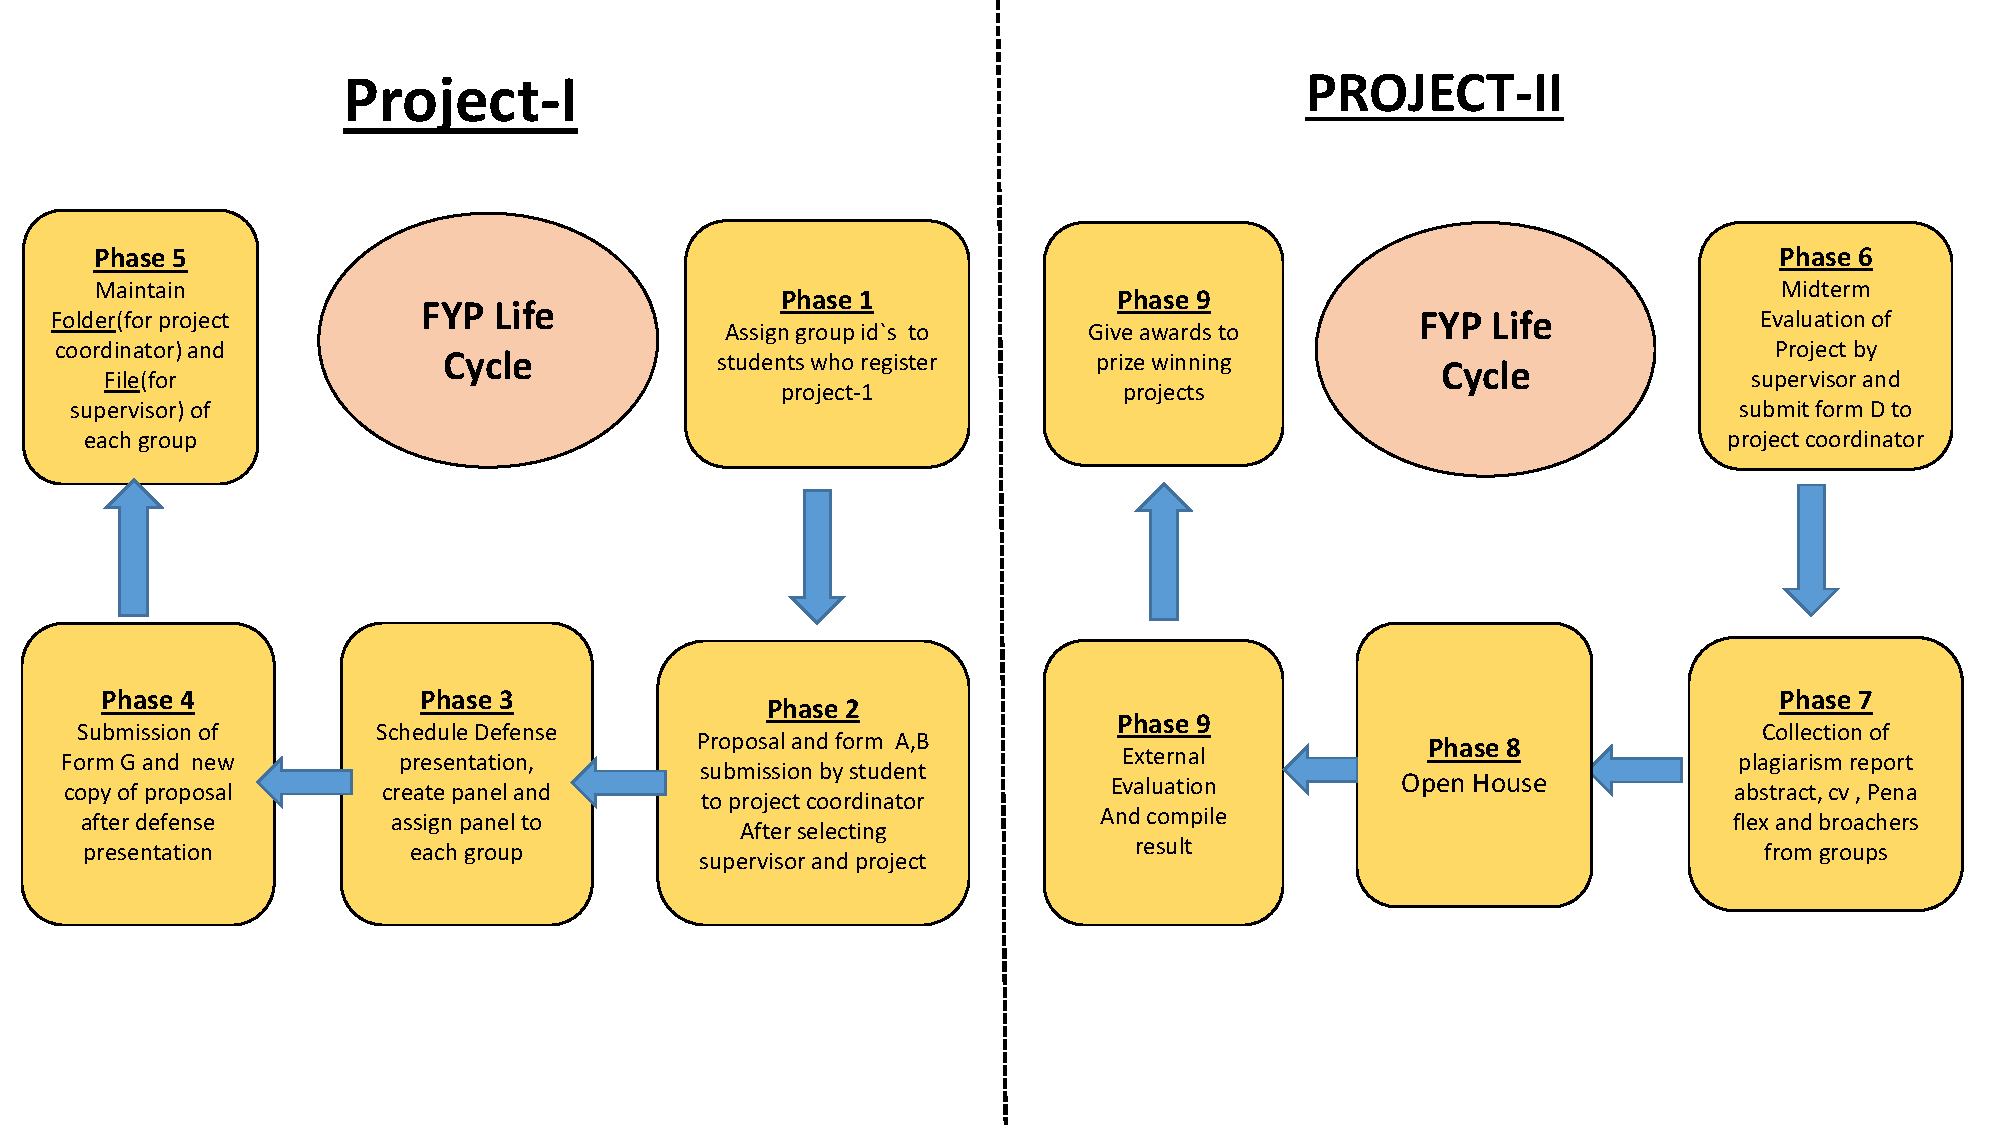
\includegraphics[scale=0.4]{fypLifeCycle}
\caption{Final Year Project Lifecycle}
\label{fig:fypLifeCycle}
\end{figure}

%%more details about figures can be found on https://en.wikibooks.org/wiki/LaTeX/Floats,_Figures_and_Captions
 
\chapter{Literature Review} \label{chap:literatureReview}

%\version{v1.10.2015}

\section*{}
Literature review is a systematic method of identifying, evaluating and interpreting the work (similar to yours) produced by others. This chapter should set the project into context and give the proposed layout for achieving the project goals. It is an important chapter especially if the project involves significant amount of ground work. Review prior work critically, identify gaps in knowledge/areas of application and build an argument for your own work. When referring to other pieces of work, cite the sources where they are referred to or used, rather than just listing them at the end. 


\chapter{Requirement Specifications} \label{chap:reqs}

%\version{v1.10.2015}

\section*{}
In this chapter, first describe the existing system, its limitations or drawbacks and then explain how the new or proposed system will overcome these problems. This should then be followed by complete requirements specification for the proposed system.  Describe the behavior of the system to be developed and include a set of use cases that describe interactions the users will have with the system. In addition also describe non-functional requirements. Non-functional requirements impose constraints on the design or implementation (such as performance engineering requirements, quality standards, or design constraints). Should have the following headings:
\begin{itemize}
	\item Existing System
	\item Proposed System
	\item Requirement Specifications
	\item Use Cases
\end{itemize}
 


\chapter{Design} \label{chap:design}

%\version{v1.10.2015}

\section*{}

Systems design is the process of defining the architecture, components, modules, interfaces, and data for a system to satisfy specified requirements. This chapter should have the following sections:

\section{System Architecture}
This section describes the system in narrative form using non-technical terms.  It should provide a high-level system architecture diagram showing a subsystem breakout of the system, if applicable.  The high-level system architecture or subsystem diagrams should, if applicable, show interfaces to external systems.  Supply a high-level context diagram for the system and subsystems, if applicable.  
\section{Design Constraints}

This section describes any constraints in the system design (reference any trade-off analyses conducted such, as resource use versus productivity, or conflicts with other systems) and includes any assumptions made during the developing the system design.
\section{Design Methodology}

Summarize the approach that will be used to create and evolve the designs for this system. Cover any processes, conventions, policies, techniques or other issues which will guide design work. This is for deciding whether you will use structured, object-oriented or other specific methodologies.  Most people will use some object-oriented technique with UML.
\section{High Level Design}
This section describes in further detail elements discussed in the Architecture. 
High-level designs are most effective if they attempt to model groups of system elements from a number of different views.  Typical viewpoints are: 
\begin{enumerate}
	\item   Conceptual or Logical: This view shows the logical functional elements of the system.  Each component represents a similar grouping of functionality.  For UML, this would be a component diagram or a package diagram.
	\item   Process:  this view is the runtime view of the system.  The components are threads or processes or distributed applications.  In UML, this would be a process interaction diagram.
	\item   Physical:  this view is for distributed systems. The components are physical processors that have parts of the system running on them.  For UML, this would be a deployment diagram.
	\item   Module:  this view is for project management and code organization.  The components are typically files or directories.  This picture shows how the directory structure of the build and development environment will be designed.
	\item   Security: this view typically focuses on the components that cooperate to provide security features of the system.  It is often a subset of the Conceptual view.
\end{enumerate}

\section{Low Level Design}
This section provides low-level design descriptions that directly support construction of modules. Normally this section would be split into separate documents for different areas of the design.  For each component we now need to break it down into its fundamental units or modules.  For an OO implementation in Java, our components would become packages.  Then the low level design will take each package and break it down into its classes.  For smaller systems, you may have a single UML class diagram that each module description refers to.

\section{Database Design}
The section should reveal the final design of all database management system (DBMS) files and the non-DBMS files associated with the system under development.  Provide a comprehensive data dictionary showing data element name, type, length, source, validation rules, maintenance (create, read, update, delete capability), data stores, outputs, aliases, and description.

\section{GUI Design}
This section provides the detailed design of the system and subsystem inputs and outputs relative to the user.  Depending on the particular nature of the project, it may be appropriate to repeat these sections at both the subsystem and design module levels.  

\section{External Interfaces}
External systems are any systems that are not within the scope of the system under development.  In this section, describe the electronic interface(s) between this system and each of the other systems and/or subsystem(s), emphasizing the point of view of the system being developed.



\chapter{System Implementation} \label{chap:sysImplementation}
%\version{v1.10.2015}

\section*{}
Implementation is the process of moving an idea from concept to reality. The System implementation is a realization of a technical specification or algorithm as a program, software component, or other computer system through programming and deployment.

\section{System Architecture}
Describe the architecture e.g. in terms of:  System internal components, Functionality of the components, Communication between the components
Tools and Technology Used
Development Environment/Languages Used
Processing Logic/Algorithms
Application Access Security
Describe new application access related security measures, e.g. in terms of: Security Zones/Firewalls, Encryption, Authentication, e.g. Account \& Password structures and rules, Authorization, e.g. operator rights and roles, authority handling, Auditing / Access Logging, Safe Data Storage
Database Security

Describe new DB related security measures, e.g. in terms of:  Remote Access, Authentication (Account \& Password: structure, rules), Authorization (rights/roles, handling), Anonymous and Group Users, Auditing/Logging (events, data, log handling).

 

\chapter{System Testing and Evaluation}\label{chap:testingEvaluation}

%\version{v1.11.2015}

\section*{}
System testing of software or hardware is testing conducted on a complete, integrated system to evaluate the system's compliance with its specified requirements. Be warned that many projects fall down through poor evaluation. Simply building a system and documenting its design and functionality is not enough to gain top marks. It is extremely important that you evaluate what you have done both in absolute terms and in comparison with existing techniques, software, hardware etc. This might involve quantitative evaluation and qualitative evaluation such as expressibility, functionality, ease-of-use etc. At some point you should also evaluate the strengths and weaknesses of what you have done. Avoid statements like "The project has been a complete success and we have solved all the problems associated with ...! It is important to understand that there is no such thing as a perfect project. Even the very best pieces of work have their limitations and you are expected to provide a proper critical appraisal of what you have done. The following are different types of testing that should be considered during System testing:

\begin{itemize}
	\item Graphical user interface testing
	\item Usability testing
	\item Software performance testing
	\item Compatibility testing
	\item Exception handling
	\item Load testing
	\item Security testing
	\item Installation testing
\end{itemize}

For research based projects this chapter should include complete description of evaluation metrics and analysis/discussion of evaluation results.

\chapter{Conclusions}\label{chap:conclusions}
%\version{v1.10.2015}

\section*{}
The project's conclusions should list the things which have been learnt as a result of the work you have done. For example, "The use of overloading in C++ provides a very elegant mechanism for transparent parallelisation of sequential programs". Avoid tedious personal reflections like "I learned a lot about C++ programming..." It is common to finish the report by listing ways in which the project can be taken further. This might, for example, be a plan for doing the project better if you had a chance to do it again, turning the project deliverables into a more polished end product.



%\chapter{Chapter 8 title} \label{chap:concl}
%\version{v1.10.2015}
\section*{}
\lipsum

\section{Sec}
\lipsum
%%\printindex
%% comment next 2 commands if numbered appendixes not used
\appendix
\chapter{User Manual} \label{ap:Appendix1}

\section*{}
Appendices are provided to give supplementary information, which is included in the main text may serve as a distraction and cloud the central theme.

\begin{itemize}
	\item Appendices should be numbered using alphabets, e.g. Appendix A, Appendix B, etc.
	\item Tables and References appearing in appendices should be numbered and referred to at appropriate places just as in the case of chapters.
	\item Appendices shall carry the title of the work reported and the same title
shall be written in the contents page.
\end{itemize}
%\chapter{Appendix} \label{ap:appendix2}

\section*{}


%%----------------------------------------
%% Final materials
%%----------------------------------------

\begin{singlespace}
  %% Bibliography
  %% comment the next command if BibTeX file not used
  %% bibliography is in ``references.bib''
  \PrintBib{references}

  %% Index
  %% uncomment next command if index is required
  %% don't forget to run ``makeindex tese'' command
  \PrintIndex
\end{singlespace}

\end{document}